\documentclass[journal]{IEEEtran}


\usepackage[pdftex]{graphicx}
\usepackage{amsmath}
\usepackage{algorithm}
\usepackage[noend]{algpseudocode}
\usepackage{array}

% correct bad hyphenation here
\hyphenation{op-tical net-works semi-conduc-tor}


\begin{document}
%
% paper title
% Titles are generally capitalized except for words such as a, an, and, as,
% at, but, by, for, in, nor, of, on, or, the, to and up, which are usually
% not capitalized unless they are the first or last word of the title.
% Linebreaks \\ can be used within to get better formatting as desired.
% Do not put math or special symbols in the title.
\title{Detection and Instance Segmentation of Neuroblastoma Cells using YOLO, UNet and Conditional Random Fields}

\author{Kristofer delas Pe\~nas and
        Dominic Waithe}% <-this % stops a space

% The paper headers
\markboth{Oxford-Nottingham Centre for Doctoral Training for Biomedical Imaging}%
{delas Pe\~nas: Detection and Semantic Segmentation of Neuroblastoma Cells using YOLO, UNet and Conditional Random Fields}
% The only time the second header will appear is for the odd numbered pages
% after the title page when using the twoside option.
% 
% *** Note that you probably will NOT want to include the author's ***
% *** name in the headers of peer review papers.                   ***
% You can use \ifCLASSOPTIONpeerreview for conditional compilation here if
% you desire.




% If you want to put a publisher's ID mark on the page you can do it like
% this:
%\IEEEpubid{0000--0000/00\$00.00~\copyright~2015 IEEE}
% Remember, if you use this you must call \IEEEpubidadjcol in the second
% column for its text to clear the IEEEpubid mark.



% use for special paper notices
%\IEEEspecialpapernotice{(Invited Paper)}




% make the title area
\maketitle

% As a general rule, do not put math, special symbols or citations
% in the abstract or keywords.
\begin{abstract}
The abstract goes here.
\end{abstract}

% Note that keywords are not normally used for peerreview papers.
\begin{IEEEkeywords}
IEEE, IEEEtran, journal, \LaTeX, paper, template.
\end{IEEEkeywords}






% For peer review papers, you can put extra information on the cover
% page as needed:
% \ifCLASSOPTIONpeerreview
% \begin{center} \bfseries EDICS Category: 3-BBND \end{center}
% \fi
%
% For peerreview papers, this IEEEtran command inserts a page break and
% creates the second title. It will be ignored for other modes.
\IEEEpeerreviewmaketitle



\section{Introduction}
\IEEEPARstart{T}{his} demo file is intended to serve as a ``starter file''
for IEEE journal papers produced under \LaTeX\ using
IEEEtran.cls version 1.8b and later.
% You must have at least 2 lines in the paragraph with the drop letter
% (should never be an issue)
I wish you the best of success.

\section{Literature Review}
\subsection{Semantic Segmentation}
\subsection{Instance Segmentation}
\subsection{YOLO}
The YOLO (You Only Look Once) network \cite{redmon2016yolo9000} is a state-of-the-art object detection system that gained popularity within the past few years. It employs a series of convolutions to detect and localize objects in real-time.

The implementation of YOLO starts with an initial 416 $\times$ 416 image input. The system performs 19 convolutions with an overall downsampling factor of 32, resulting to an output feature map of 13 $\times$ 13 dimension which is used to predict the bounding boxes of detected objects with the help of anchor boxes.

With version 2 of YOLO, \cite{redmon2016yolo9000} demonstrated a high mean average precision (mAP) on the VOC dataset, higher than existing architectures like Faster-RCNN.

A more recent YOLO iteration, version 3 \cite{yolov3}, uses a deeper network and performs object detection on 3 stages of different resolutions. With these changes, an even higher mAP was achieved, however, at the expense of heavier computational resource requirement and longer detection time.
\subsection{UNet}
UNet\cite{RFB15a} is a fully convolutional neural network architecture that aims to semantically label individual pixels in the image. The network consists of two paths - a contracting path and an expansive path. The contracting path is the typical convolutional network with a series of convolutional layers with rectified linear unit (ReLU) activations and pooling layers to downsample.

The expansive path is an upsampling route, taking the output of the previous path. This path performs a series of \textit{up-convolutions}, a combination of upsampling and a 2 $\times$ 2 convolution.

The key feature in UNet is the shortcut connections between the two paths for each resolution scale as shown in Figure \ref{fig:unet}. At each scale, concatenating the output from the contracting path with the upsampled output from the previous scale in the expansive path, ensures that the finer details lost through downsampling can be recovered and be used to fine tune the segmentation.

UNet was first applied on microscopy images but since then have been applied to different imaging modalities like MRIs and CT scans.
\begin{figure}
\centering
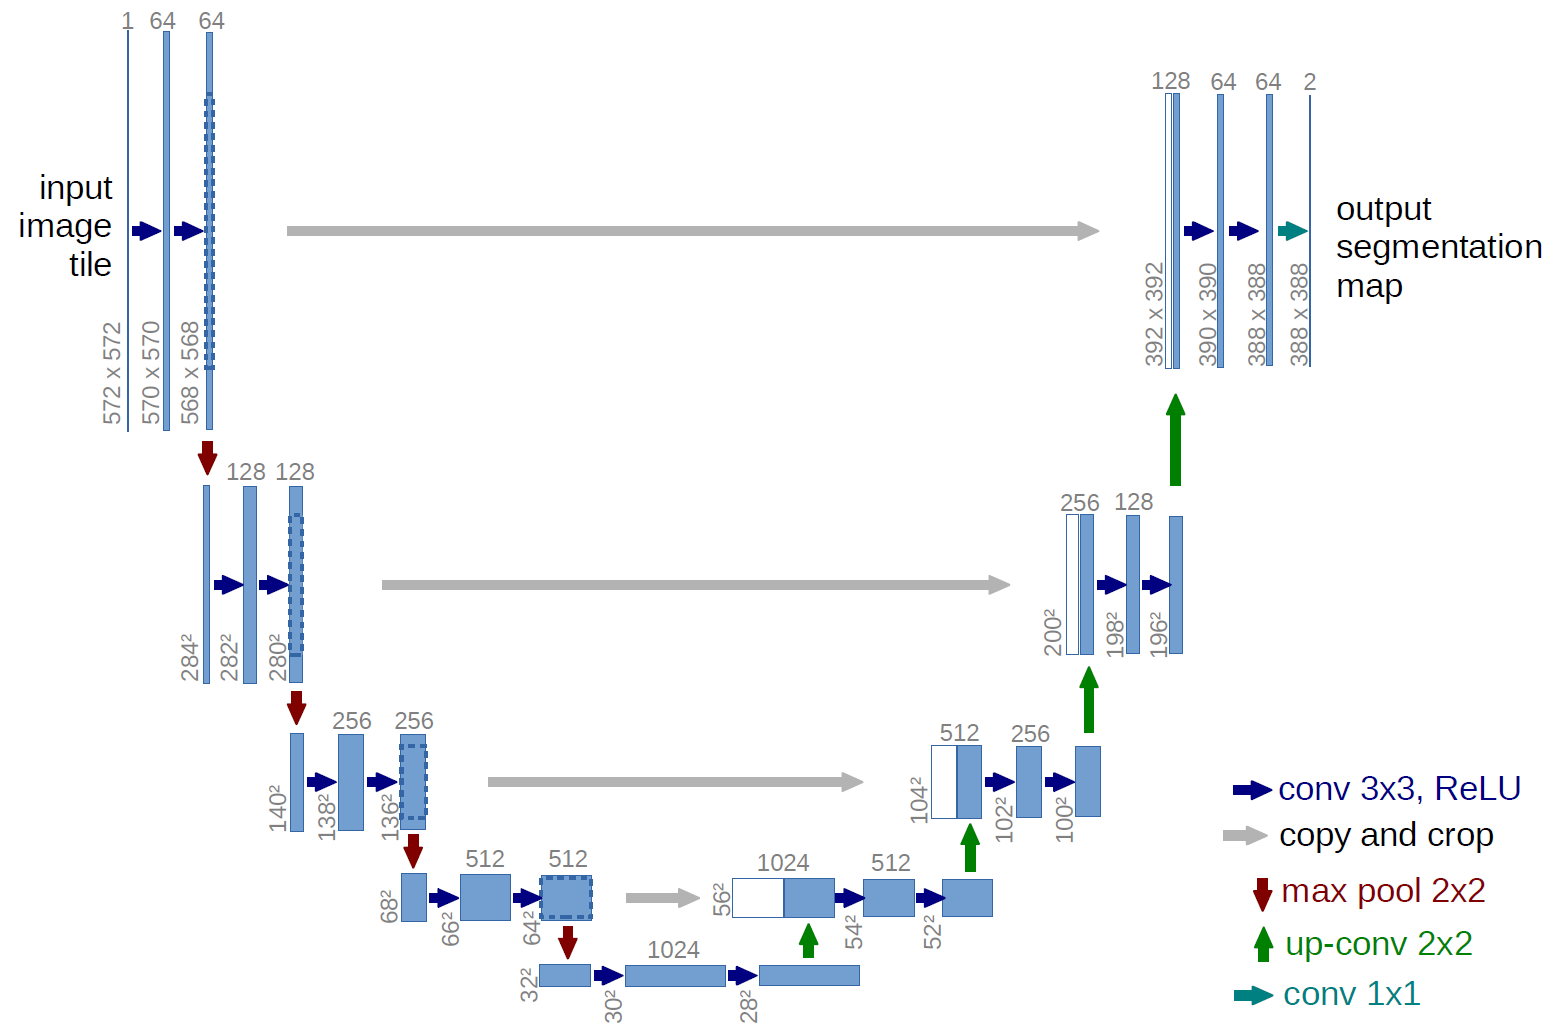
\includegraphics[width=3in]{unet.png}
\caption{\textbf{U-net architecture} \cite{RFB15a} (example for 32x32 pixels in the lowest resolution). Each blue
box corresponds to a multi-channel feature map. The number of channels is denoted
on top of the box. The x-y-size is provided at the lower left edge of the box. White
boxes represent copied feature maps. The arrows denote the different operations.}
\label{fig:unet}
\end{figure}
\subsection{Conditional Random Fields}
Many learning problems can be described as a graphical model. In artificial intelligence, one common way to model these problems is a probabilistic approach wherein probability distributions \textit{$\Psi$} are assigned over the random variables \textit{Y}. Formally, the problem can be modelled as the product of all \textit{$\Psi_i$} distributions
\begin{equation}
p(Y) = \frac{1}{Z}\prod_1^A \Psi_a(y_a)
\end{equation}
for factors \textit{F} = \{$\Psi_a$\} that have $\Psi_a \geq 0$. 
 
Markov networks and conditional random fields (CRF) are formulated similarly in this manner. The main difference is that the CRF learns the conditional probability $p(y|x)$ while Markov networks ultimately obtain the joint probability $p(y,x)$. With the joint probability $p(y,x)$, models like the Markov networks can describe the hypothesis space through the generation of all possible features \textit{x} for all labels \textit{y}. However, joint probability $p(y,x)$ involves prior knowledge on or estimate for $p(x)$, and the dependence (or independence) of the random variables. For general classification tasks, however, modelling of $p(x)$ is not needed as the concern is only on assigning labels to features, which is exactly what the conditional probability $p(y|x)$ gives.

%put figure here
Exact inference on conditional random fields is computationally expensive and usually impossible. If exact inference is possible, performing naively the sum of products of potentials (\textbf{message passing}) for all variables, can take a long time, especially for dense graphs. Current implementations of CRFs perform inference by approximation, with the speedup by employing dynamic programming. One inference algorithm is the mean field inference described in Algorithm \ref{alg:meanfieldinference}.

Each iteration of the mean field inference described in Algorithm \ref{alg:meanfieldinference} performs a message passing step, compatibility transform, and local update and normalization. Each step, except the message passing, runs in linear time. Message passing is the computational bottleneck. For a naive solution, it requires summing up over all variables and runs in quadratic time. For this very reason, the conditional random fields gained the reputation of being nooriously slow and impractical for a lot of machine learning tasks, especially those involving dense graph representations like image segmentation.

%message passing as convolution
Addressing the slow inference in CRFs, \cite{NIPS2011_4296} showed that message passing can be approximated and expressed as a convolution with a Gaussian kernel as follows:
\begin{equation}
\widetilde{Q}_i^{(m)}(l)\gets \sum_{j\neq i}k^{(m)}(f_i,f_j)Q_j(l) = [G_(m) \otimes Q(l)](f_i) - Q_i(l)
\end{equation}
This approximation can be extended to higher dimensions, and with the permutohedral lattice data structure, efficient message passing can be done in $O(Nd)$ time where \textit{N} is the number of variables and \textit{d} the number of dimensions. 
%cnnasrnn
Furthermore, \cite{crfasrnn_ICCV2015} and \cite{higherordercrf_ECCV2016} demonstrated how the mean field inference in CRFs can be written as recurrent neural network with learnable weights. This formulation allows the CRFs to be seamlessly integrated as part of a convolutional neural network model for tasks such as image segmentation.

With CRFs implemented as RNNs, several research has been done applying CNN-CRFs for general image segmentation task. \cite{NIPS2011_4296} and \cite{Teichmann2018ConvolutionalCF} proposed systems using CRFs integrated in CNNs for semantic image segmentation. Both systems train the CRF by minimizing the Gibbs energy and in doing so, finding the Maximum A Posteriori labelling of the image pixels. The CRF for semantic image segmentation is formulated with the following energy function for assignment of the pixels to semantic classes,
\begin{equation}
E(X = x) = \sum_i U(x_i) + \sum_{i<j}P(x_i,x_j)
\end{equation}
where \textit{U} is the unary potential and \textit{P} the pairwise potential. In \cite{NIPS2011_4296}, responses from the TextonBoost filter bank, color, histogram of oriented gradients (HOG) and pixel location features were used for the unary potential. On the other hand, \cite{Teichmann2018ConvolutionalCF} used the segmentation prediction from ResNet101 for the unary. Both systems used gaussian kernels for the pairwise potentials, given as:
\begin{equation}
k(f_i^I,f_j^I) = w^{(1)}G_{appearance} + w^{(2)}G_{smoothness}
\end{equation}
\begin{equation}
G_{appearance} = exp\left(-\frac{|p_i - p_j|^2}{2\theta_\alpha^2} - \frac{|I_i - I_j|^2}{2\theta_\beta^2}\right)
\end{equation}
\begin{equation}
G_{smoothness} = exp\left(-\frac{|p_i - p_j|^2}{2\theta_\gamma^2}\right)
\end{equation}
The two terms in the pairwise potential encourages neighboring pairs of pixels that look similar to be assigned the same semantic label.

Extending from this, \cite{Arnab2017PixelwiseIS} and \cite{Li_2018_ECCV} introduced some modification to this energy function to be able to perform  pixelwise instance segmentation. The systems described for this task works on an initial instance segmentation from a detection algorithm, where each detection has a corresponding prediction score. This instance segmentation is further refined by adding information from semantic segmentation and the gaussian pairwise potentials. To do this, They have broken down the unary potential to accommodate two distinct terms $\Psi_{box}$ and $\Psi_{global}$ as follows:
\begin{equation}
U(x_i) = -ln[w_1\Psi_{box}(x_i) + w_2\Psi_{global}(x_i)]
\end{equation}
The $\Psi_{box}$ term encourages the pixel to be assigned to the instance corresponding to the detection. This is proportional to the probability of the semantic class assigned to the pixel and the detection score. The $\Psi_{global}$ term accounts for pixels that might have been misclassified to another instance label but belongs to the same semantic label. This addresses the problem in the initial instance segmentation that does not fully cover the entire extent of the individual instances.
\begin{algorithm*}
\caption{Mean Field Inference}\label{alg:meanfieldinference}
\begin{algorithmic}[1]
\State Initialize $Q$
\While{not converged}
\State $\widetilde{Q}_i^{(m)}(l)\gets \sum_{j\neq i}k^{(m)}(f_i,f_j)Q_j(l)$ for all m\Comment{Message Passing}
\State $\hat{Q}_i(x_i)\gets \sum_{l \in L} \mu^{(m)}(x_i,l)\sum_w^{(m)}\widetilde{Q}_i^{(m)}(l)$
\State $Q_i(x_i)\gets exp{-\psi_u(x_i) - \hat{Q}_i(x_i)}$
\State normalize $Q_i(x_i)$
\EndWhile
\State \textbf{end while}
\end{algorithmic}
\end{algorithm*}

% needed in second column of first page if using \IEEEpubid
%\IEEEpubidadjcol


% An example of a floating figure using the graphicx package.
% Note that \label must occur AFTER (or within) \caption.
% For figures, \caption should occur after the \includegraphics.
% Note that IEEEtran v1.7 and later has special internal code that
% is designed to preserve the operation of \label within \caption
% even when the captionsoff option is in effect. However, because
% of issues like this, it may be the safest practice to put all your
% \label just after \caption rather than within \caption{}.
%
% Reminder: the "draftcls" or "draftclsnofoot", not "draft", class
% option should be used if it is desired that the figures are to be
% displayed while in draft mode.
%
%\begin{figure}[!t]
%\centering
%\includegraphics[width=2.5in]{myfigure}
% where an .eps filename suffix will be assumed under latex, 
% and a .pdf suffix will be assumed for pdflatex; or what has been declared
% via \DeclareGraphicsExtensions.
%\caption{Simulation results for the network.}
%\label{fig_sim}
%\end{figure}

% Note that the IEEE typically puts floats only at the top, even when this
% results in a large percentage of a column being occupied by floats.


% An example of a double column floating figure using two subfigures.
% (The subfig.sty package must be loaded for this to work.)
% The subfigure \label commands are set within each subfloat command,
% and the \label for the overall figure must come after \caption.
% \hfil is used as a separator to get equal spacing.
% Watch out that the combined width of all the subfigures on a 
% line do not exceed the text width or a line break will occur.
%
%\begin{figure*}[!t]
%\centering
%\subfloat[Case I]{\includegraphics[width=2.5in]{box}%
%\label{fig_first_case}}
%\hfil
%\subfloat[Case II]{\includegraphics[width=2.5in]{box}%
%\label{fig_second_case}}
%\caption{Simulation results for the network.}
%\label{fig_sim}
%\end{figure*}
%
% Note that often IEEE papers with subfigures do not employ subfigure
% captions (using the optional argument to \subfloat[]), but instead will
% reference/describe all of them (a), (b), etc., within the main caption.
% Be aware that for subfig.sty to generate the (a), (b), etc., subfigure
% labels, the optional argument to \subfloat must be present. If a
% subcaption is not desired, just leave its contents blank,
% e.g., \subfloat[].


% An example of a floating table. Note that, for IEEE style tables, the
% \caption command should come BEFORE the table and, given that table
% captions serve much like titles, are usually capitalized except for words
% such as a, an, and, as, at, but, by, for, in, nor, of, on, or, the, to
% and up, which are usually not capitalized unless they are the first or
% last word of the caption. Table text will default to \footnotesize as
% the IEEE normally uses this smaller font for tables.
% The \label must come after \caption as always.
%
%\begin{table}[!t]
%% increase table row spacing, adjust to taste
%\renewcommand{\arraystretch}{1.3}
% if using array.sty, it might be a good idea to tweak the value of
% \extrarowheight as needed to properly center the text within the cells
%\caption{An Example of a Table}
%\label{table_example}
%\centering
%% Some packages, such as MDW tools, offer better commands for making tables
%% than the plain LaTeX2e tabular which is used here.
%\begin{tabular}{|c||c|}
%\hline
%One & Two\\
%\hline
%Three & Four\\
%\hline
%\end{tabular}
%\end{table}


% Note that the IEEE does not put floats in the very first column
% - or typically anywhere on the first page for that matter. Also,
% in-text middle ("here") positioning is typically not used, but it
% is allowed and encouraged for Computer Society conferences (but
% not Computer Society journals). Most IEEE journals/conferences use
% top floats exclusively. 
% Note that, LaTeX2e, unlike IEEE journals/conferences, places
% footnotes above bottom floats. This can be corrected via the
% \fnbelowfloat command of the stfloats package.




\section{Conclusion}
The conclusion goes here.





% if have a single appendix:
%\appendix[Proof of the Zonklar Equations]
% or
%\appendix  % for no appendix heading
% do not use \section anymore after \appendix, only \section*
% is possibly needed

% use appendices with more than one appendix
% then use \section to start each appendix
% you must declare a \section before using any
% \subsection or using \label (\appendices by itself
% starts a section numbered zero.)
%


\appendices
\section{Proof of the First Zonklar Equation}
Appendix one text goes here.

% you can choose not to have a title for an appendix
% if you want by leaving the argument blank
\section{}
Appendix two text goes here.


% use section* for acknowledgment
\section*{Acknowledgment}


The authors would like to thank...


% Can use something like this to put references on a page
% by themselves when using endfloat and the captionsoff option.
\ifCLASSOPTIONcaptionsoff
  \newpage
\fi



% trigger a \newpage just before the given reference
% number - used to balance the columns on the last page
% adjust value as needed - may need to be readjusted if
% the document is modified later
%\IEEEtriggeratref{8}
% The "triggered" command can be changed if desired:
%\IEEEtriggercmd{\enlargethispage{-5in}}

% references section

% can use a bibliography generated by BibTeX as a .bbl file
% BibTeX documentation can be easily obtained at:
% http://mirror.ctan.org/biblio/bibtex/contrib/doc/
% The IEEEtran BibTeX style support page is at:
% http://www.michaelshell.org/tex/ieeetran/bibtex/
%\bibliographystyle{IEEEtran}
% argument is your BibTeX string definitions and bibliography database(s)
\bibliographystyle{IEEEtran}
\bibliography{ONBI_ROTATION_PROJECT1_DELASPENAS}
%
% <OR> manually copy in the resultant .bbl file
% set second argument of \begin to the number of references
% (used to reserve space for the reference number labels box)

% biography section
% 
% If you have an EPS/PDF photo (graphicx package needed) extra braces are
% needed around the contents of the optional argument to biography to prevent
% the LaTeX parser from getting confused when it sees the complicated
% \includegraphics command within an optional argument. (You could create
% your own custom macro containing the \includegraphics command to make things
% simpler here.)
%\begin{IEEEbiography}[{\includegraphics[width=1in,height=1.25in,clip,keepaspectratio]{mshell}}]{Michael Shell}
% or if you just want to reserve a space for a photo:

\begin{IEEEbiography}{Michael Shell}
Biography text here.
\end{IEEEbiography}

% if you will not have a photo at all:
\begin{IEEEbiographynophoto}{John Doe}
Biography text here.
\end{IEEEbiographynophoto}

% insert where needed to balance the two columns on the last page with
% biographies
%\newpage

\begin{IEEEbiographynophoto}{Jane Doe}
Biography text here.
\end{IEEEbiographynophoto}

% You can push biographies down or up by placing
% a \vfill before or after them. The appropriate
% use of \vfill depends on what kind of text is
% on the last page and whether or not the columns
% are being equalized.

%\vfill

% Can be used to pull up biographies so that the bottom of the last one
% is flush with the other column.
%\enlargethispage{-5in}



% that's all folks
\end{document}


